\section{分类汇总}

​在表格中实现简单的统计分析工作，相信大家第一时间肯定会想到使用函数公式，或者是数据透视表。其实，Excel中还有一个非常实用的功能，能帮助你快速实现表格的多级统计，它的名字叫分类汇总。

接下来，我们就来学习分类汇总的使用方法。

看下面这个案例，需要快速统计出每天的服务人数总和，以及每天每个组别的平均服务时长，我们可以使用分类汇总功能来实现。

\begin{figure}[htpb]
    \centering
    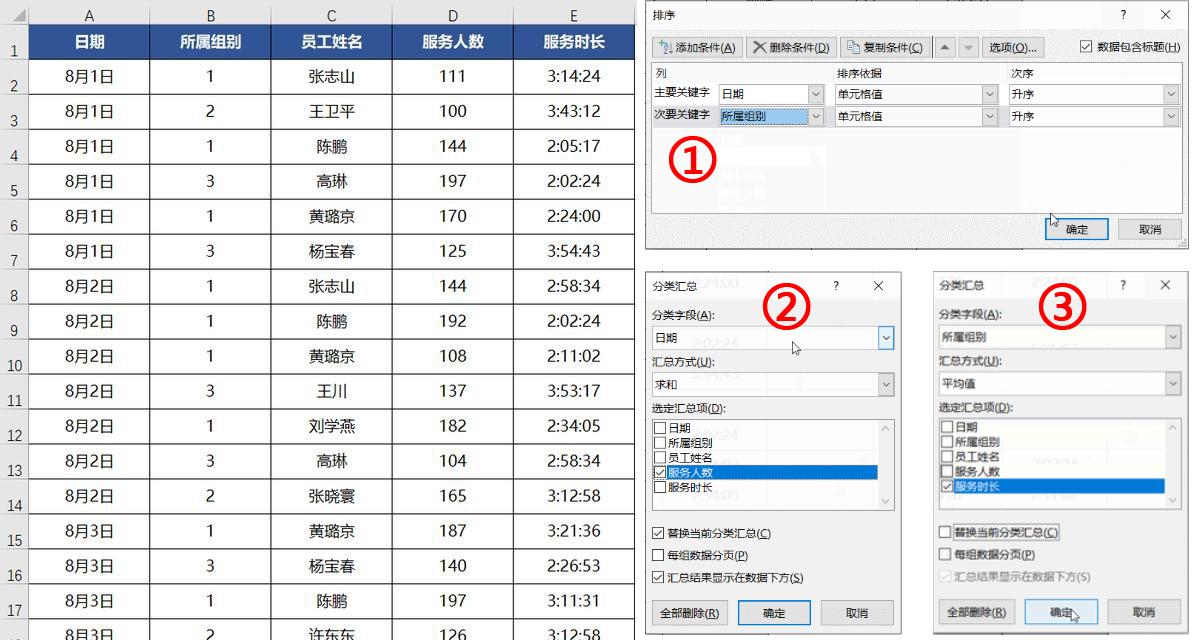
\includegraphics[width=\linewidth]{figures/classify.png}
\end{figure}

\begin{enumerate}
    \item 先对汇总条件进行排序
    
    统计的条件有两个，分别是日期和组别，我们使用自定义排序功能，添加排序条件，主要关键字选择【日期】，次序选择【升序】；次要关键字选择【所属组别】，次序选择【升序】，完成对数据的排序。
    \item 按日期为分类做一级汇总
    
    点击打开【数据】选项卡，使用【分类汇总】功能，分类字段选择【日期】，选定汇总项勾选【服务人数】，做出一级统计。
    \item 按组别为分类做二级汇总
    
    再次使用分类汇总功能，分类字段选择【所属组别】，汇总方式选择【平均值】，选定汇总项勾选【服务时长】。

    这里需要注意的是，要把【替换当前分类汇总】的勾选去掉，才能实现二级汇总。
\end{enumerate}

实现分类汇总后，我们可以从表格中快速地看出每天每个组别的平均服务时长，以及每天的服务人数。

\begin{figure}[htpb]
    \centering
    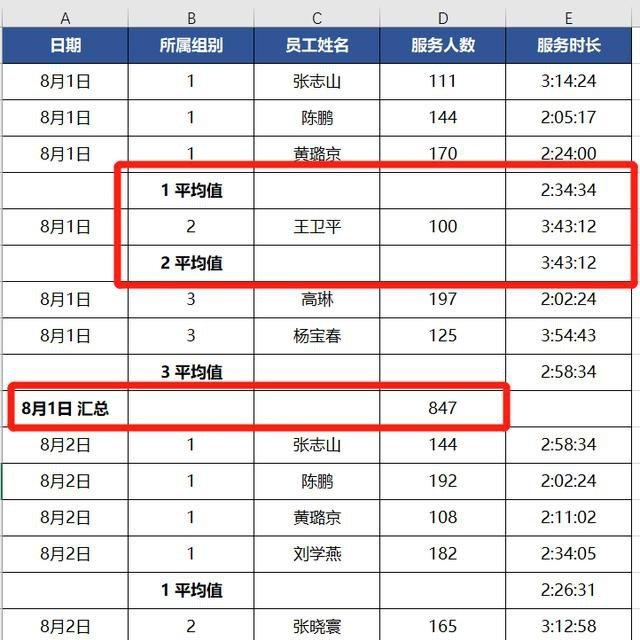
\includegraphics[width=.5\linewidth]{figures/classify1.png}
\end{figure}

点击左侧的加减号或者组别，能够折叠和展开每个层级的数据，方便查看明细数据和汇总数据。

最后，如果要删除分类汇总，重新打开分类汇总功能，点击全部删除即可。

备注：数据分类汇总与数据透视表相比，数据透视表相对灵活方便，建议实际分类汇总数据中使用数据透视表。

\section{数据透视表}

数据透视表建立在明细数据记录基础之上。集合了排序、筛选和分类汇总的功能，并生成汇总表格，集中体现了Excel强大的数据分析功能。

\begin{enumerate}
    \item 创建数据透视表
        \begin{enumerate}
            \item 选中区域，点击【插入】选项卡，点击【数据透视表】按钮，弹出【创建数据透视表】对话框
            \item 在弹出的【数据透视表字段】中，把字段拖动到相对应的【行】【列】【值】区域。
        \end{enumerate}
    \item 值汇总方式
        \begin{enumerate}
            \item 点击【值】区域中的“求和项:产量”，弹出菜单中选择【值字段设置】，弹出【值字段设置】对话框，【计算类型】进行选择
            \item 如果对数值显示方式有要求，在弹出【值字段设置】对话框，点击左下角【数字格式】进行设置。
        \end{enumerate}    
    \item 数据透视表排序
        
    点击【行标签】或【列标签】右侧倒三角按钮，选择弹出菜单栏中的【其他排序选项】，在弹出的【排序】对话框，可以选择【排序选项】中的手动、升序排序还是降序排列。
    \item 数据百分比计算
        \begin{enumerate}
            \item 再次拖动“产量”到【值】区域，“产量”字段汇总方式在【值字段设置】对话框都设置为【求和】，【值】区域内有【求和项：产量】和【求和项：产量2】
            \item 把光标放于【求和项：产量2】这一列的数字上，点击鼠标右键，弹出菜单选择【值显示方式】，在右侧列表选择“列汇总百分比”，将该列表头改为“百分比”即可。
        \end{enumerate}
    \item 从数据透视表创建数据透视图
    
    在表格中选择一个单元格。选择“数据透视表工具”>“分析”>“数据透视图”。选择图表。
\end{enumerate}

\begin{figure}[htpb]
    \centering
    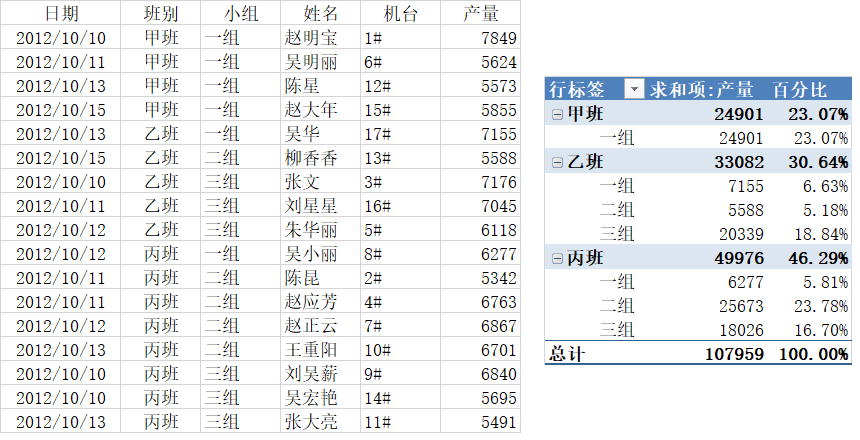
\includegraphics[width=.8\linewidth]{figures/透视表.png}
\end{figure}


\section{图表}

{\bfseries \cgreen{创建图表}}
\begin{enumerate}
    \item 选择要用于图表的数据。
    \item 单击“插入”>“推荐的图表”。
    \item 在“推荐的图表”选项卡上，滚动浏览 Excel 为您的数据推荐的图表列表，然后单击任意图表以查看数据的呈现效果。
    \item 如果没有看到您喜欢的图表，请单击“所有图表”以查看所有可用的图表类型。
    \item 找到所要的图表时，单击该图表，然后单击“确定”。
    \item 使用图表右上角附近的“图表元素”、“图表样式”和“图表筛选器”按钮添加坐标轴标题或数据标签等图表元素，自定义图表的外观或更改图表中显示的数据。
    \item 若要访问其他设计和格式设置功能，请单击图表中的任意位置将“图表工具”添加到功能区，然后在“设计”和“格式”选项卡上单击所需的选项。
\end{enumerate}

{\bfseries \cgreen{添加饼图}}

单击“插入”>“插入饼图或圆环图”，然后选择所需的图表。

饼图可以将电子表格数据的一列或一行转换到饼图中。 饼图的每个扇区（数据点）显示该扇区相对于整个饼图的大小或百分比。

最适合采用饼图的情形：
\begin{itemize}
    \item 只有一个数据系列。
    \item 任何数据值都不为零或小于零。
    \item 类别不超过七个。因为七个以上的扇区会使图表难以阅读。
\end{itemize}

除了三维饼图图表，您还可以创建复合饼图或复合条饼图。 这些图表在显示一些较小的值时，将这些值分离出来放到次饼图或堆积条形图中，从而使其更易于辨别。

{\bfseries \cgreen{分离或展开饼图}}

\begin{itemize}
    \item 分离单个扇区
\end{itemize}

选中要拉出的扇区，然后将该扇区从图表中心拖开。

\begin{itemize}
    \item 分离整个饼图
\end{itemize}

右键单击饼图，然后单击“设置数据系列格式”。拖动“饼图分离”滑块以增加分隔，或在百分比框中输入数字。

{\bfseries \cgreen{在饼图中添加或删除数据}}

\begin{itemize}
    \item 单击图表中的任意位置。当前显示的源数据在工作表上处于选中状态，其中显示了尺寸控点。在工作表中，拖动尺寸控点以包含新的数据或删除数据。
    \item 右键单击图表，然后“选择数据”。
\end{itemize}

{\bfseries \cgreen{向图表添加图例}}

大多数图表使用某种图例来帮助读者了解图表数据。 每当在 Excel 创建图表时，都会同时自动生成图表的图例。 如果图表已手动从图表中删除，则图表可能缺少图例，但可以检索丢失的图例。

单击图表。单击加号“图表元素”。选中“图例”复选框。

{\bfseries \cgreen{编辑图例文本}}

如果图表中的图例名称不正确，可以重命名图例项。

\begin{enumerate}
    \item 右键单击图表。“选择数据”。
    \item 在“系列”列表的图例项，然后单击“编辑”。
    \item 在“系列名称”字段中，键入新的图例项。
\end{enumerate}



